\documentclass[12pt]{report}
\usepackage{amsmath}
\usepackage{amssymb}
\usepackage{graphicx}
\usepackage{hyperref}
\usepackage{color}
\usepackage{float}
\begin{document}
		\title{Chromatin Architecture Post UVC damage- Summary of Results}	
		\author{Ofir Shukron, David Holcman}	
		\maketitle
	\section{Main Findings}\label{section:MainFindings}
		\begin{itemize}
			\item Post UVC chromatin undergoes conformational changes such as unpacking by breaking cross-links (CTCF, cohesin), straightening caused by repair mechanism proteins crowding and active force applied on chromatin;
			\item During crowding of repair mechanism, both DNA and histones are pushed and leave the ROI at the same proportion. 
            \item We offer a conceptual 1D model in which sliding and pushing causes loss in different proportions (Figures \ref{fig:histoneSlidingSingle}, \ref{fig:histoneSlidingMulti});
			\item We offer a formula to calculate the contribution of sliding to the radius of expansion, equation \ref{eq:expansionRadiusDueToSliding};			
			\item We offer a formula to calculate the ratio of chromatin length to the ROI radius, equation \ref{eq:ratioOfDNALengthToRoiRadius};
			\item Analysis of patch expansion data based on preservation of material in the patch(equation \ref{eq:HistonePreservationConcentric}), followed by a quadratic polynomial fit to the histone gain function shows sliding is responsible to between 0.38 to 0.46 $\mu m$ of expansion, equation ;
			\item  we validate our analysis method on UV dose dependent data
			\item To examine the organization of the  chromatin post repair, we perform simulations. We calibrate our simulation framework to 20\% loss of DNA after linkers have been removed by repair proteins, and volume of exclusion was placed around each damaged point. We slowly introduce cross-links to the levels they were before. 
			The measure of similarity is the mean number of neighbors each monomer in the ROI has relative to what it had previously
			
		\end{itemize}
		
		\section{Histone sliding model}\label{section:HistoneSlidingModel}
		   \begin{figure}[H]
		   	\centering
		   	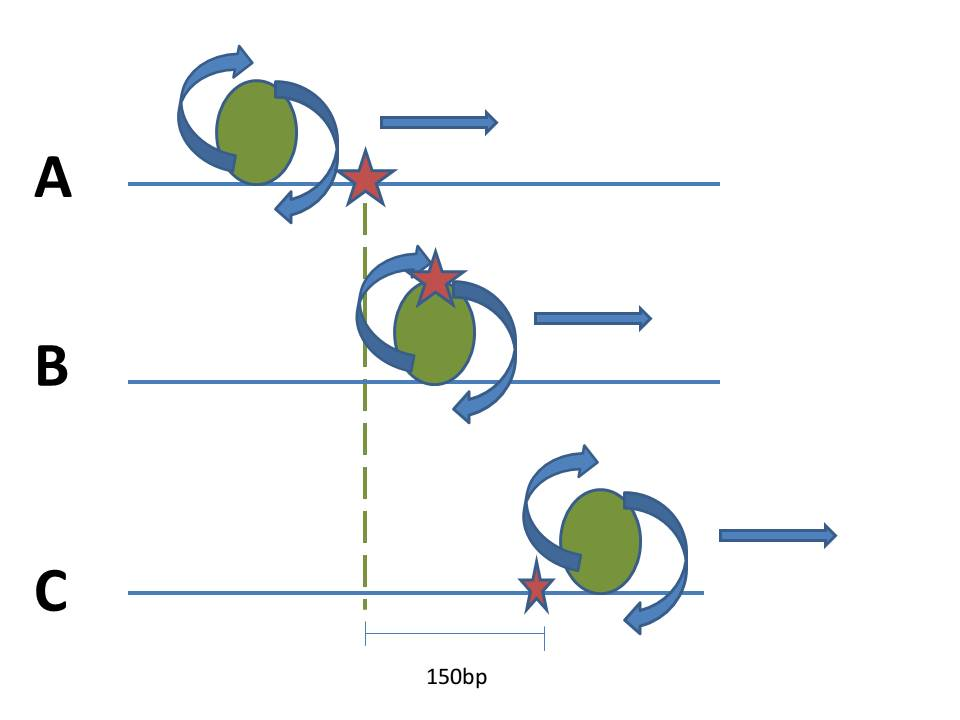
\includegraphics[width=0.7\linewidth]{Images/SlidingModel/histoneSlidingSingle}
		   	\caption{{Three time points during a displacement of damage site (red star) caused by histone rolling. The displacement of the damage site is equivalent to the length of DNA wrapped on a histone. A displacement is relative to some reference point, like the origin, and does not refer to an actual motion on the DNA}}
		   	\label{fig:histoneSlidingSingle}
		   \end{figure}
		   
		   \begin{figure}[H]
		   	\centering
		   	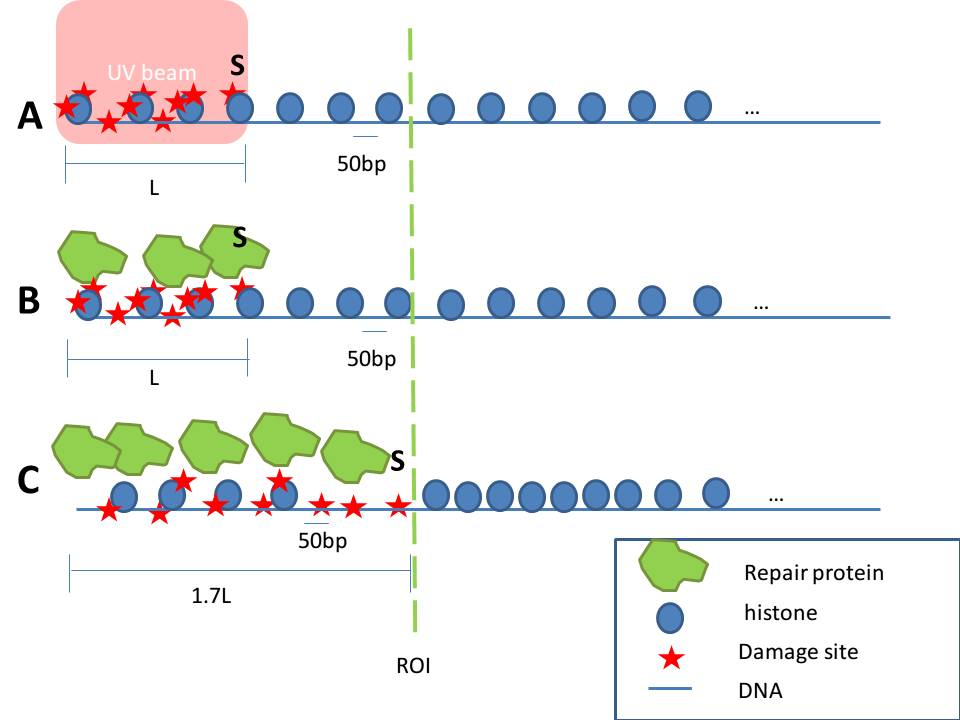
\includegraphics[width=0.7\linewidth]{Images/SlidingModel/histoneSlidingMulti}
		   	\caption{Expansion of the ROI due to nucleusome sliding. \textbf{A}. A UV beam (transparent red) damages DNA, with the point $S$ being the rightmost damage site \textbf{B}. Repair proteins (green polygons) are recruited to the damage site and expose the DNA in order the repair damages. \textbf{C}. Sliding the nucleosomes to the right in order to expose damage sites, translates the point $S$ from $S$ to $\beta$. Repair proteins follow the damage point to its new location. The presence of repair proteins in $\beta$ mark the ROI's boundary (vertical dashed green line). All DNA and histones to the right of $S$ are lost}
		   	\label{fig:histoneSlidingMulti}
		   \end{figure}
		   
		To explain the imbalance between the loss of histone and DNA we put forward a 1D histone sliding model. Histones and DNA are lost from the ROI by two sub-mechanisms, one pushing the DNA out of the ROI caused by repair mechanism crowding, and the second by sliding histones. We note that by DNA pushing is active throughout histone sliding, but not conversely.
		
		We find DNA loss fraction
		\begin{equation*}
        d=\frac{\beta-L}{\beta}
		\end{equation*}
		Histone loss fraction 
		\begin{equation*}
			h=\frac{(\beta -L)(\beta+\alpha)}{\beta l}
		\end{equation*}
		with $\beta$ the end radius of expansion, $l$ the length of DNA in the damage zone, $\alpha$ the ratio of the length of a nucleosome to the DNA wrapped around a histone, 
				
		
		
		\section{Expansion attributed to sliding and pushing sub-mechanisms}
		To estimate the relative contribution of each sub-mechanism to the total expansion of the ROI, we divide the process into two: pushing and then pushing+sliding. The composition and order of events will be neglected in this description. 
		
	    If due to pushing up to a distance of $0<L<\beta$ we have lost a fraction of $k$ of both histones and DNA, we have for the total fraction of DNA and histone loss
         
		\begin{eqnarray*}
			d &=& k+\frac{\beta-L}{\beta}(1-k) \\
			h &=& k+\frac{(\beta-L)(\beta+\alpha)}{\beta l}(1-k)
		\end{eqnarray*}
		
     	with $l$ the length of a chromatin in the damage zone, $L$ is the expansion radius attributed to pushing, $\alpha$ the ratio of the length of nucleusome to the length of DNA wrapped on a histones. 
     	
		The distance to which sliding is active is thus 
		\begin{equation}\label{eq:expansionRadiusDueToSliding}
		L = \beta- \frac{\beta l(d-1)}{l(d-1) +\pi \beta(d-h)}
		\end{equation}
		Some values for the radius attributed to either mechanism are given in the figure below
		\begin{figure}[H]
			
			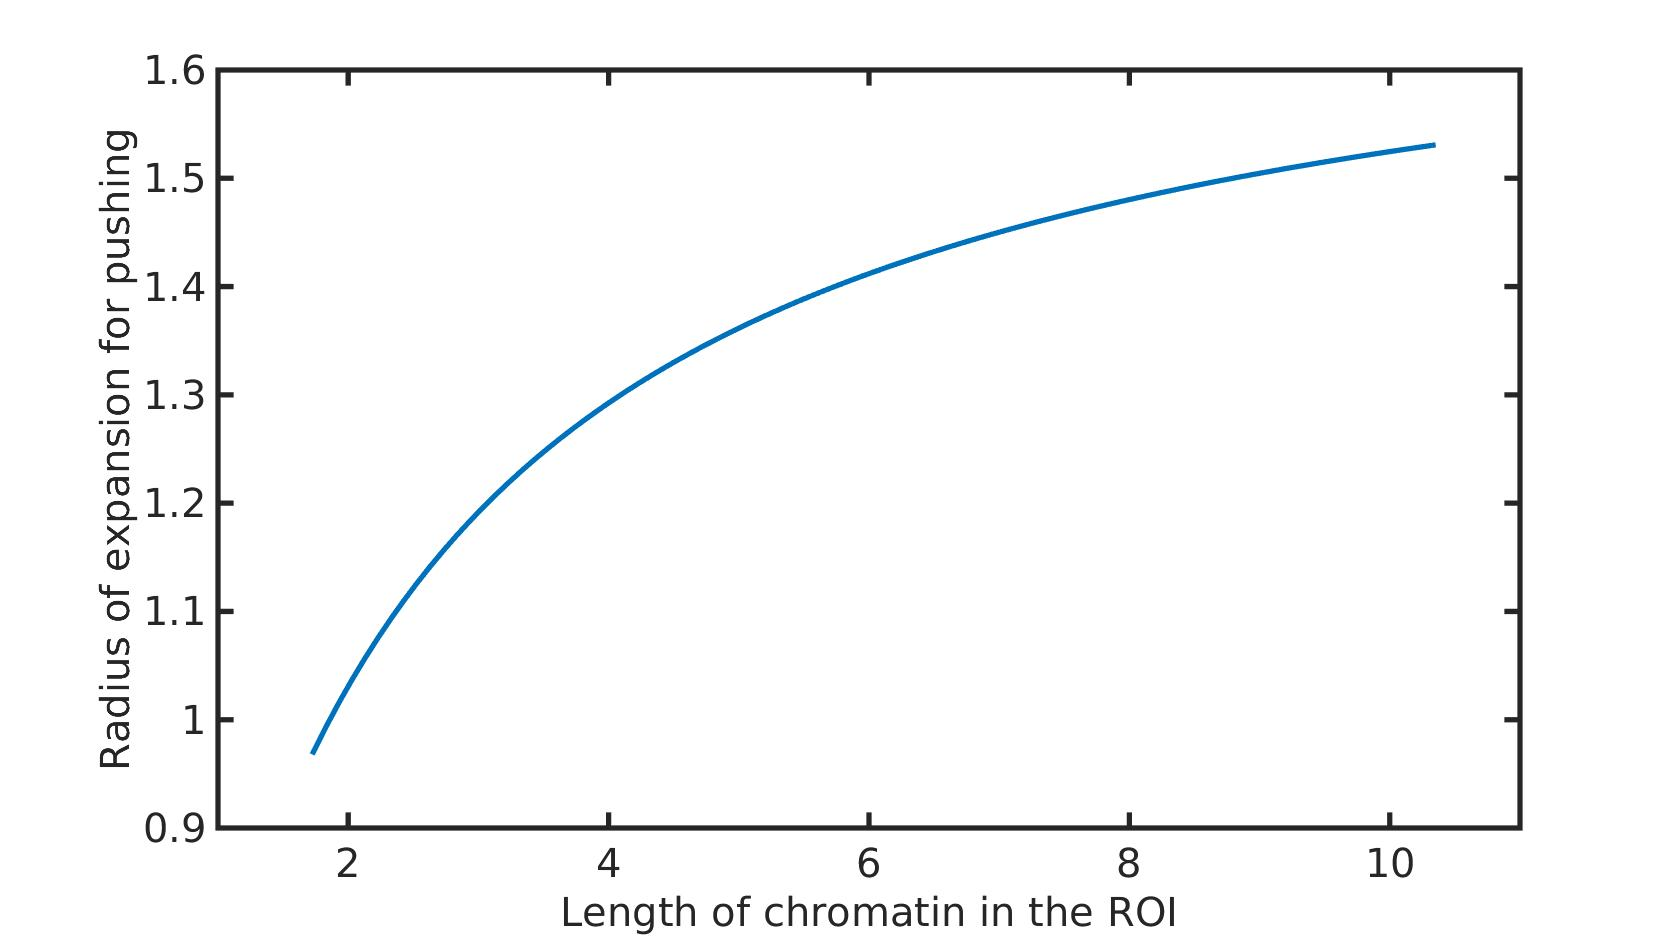
\includegraphics[width=0.5\linewidth, height=0.3\textheight]{Images/SlidingModel/radiusOfPushingVsLengthOfChromainInROI}
			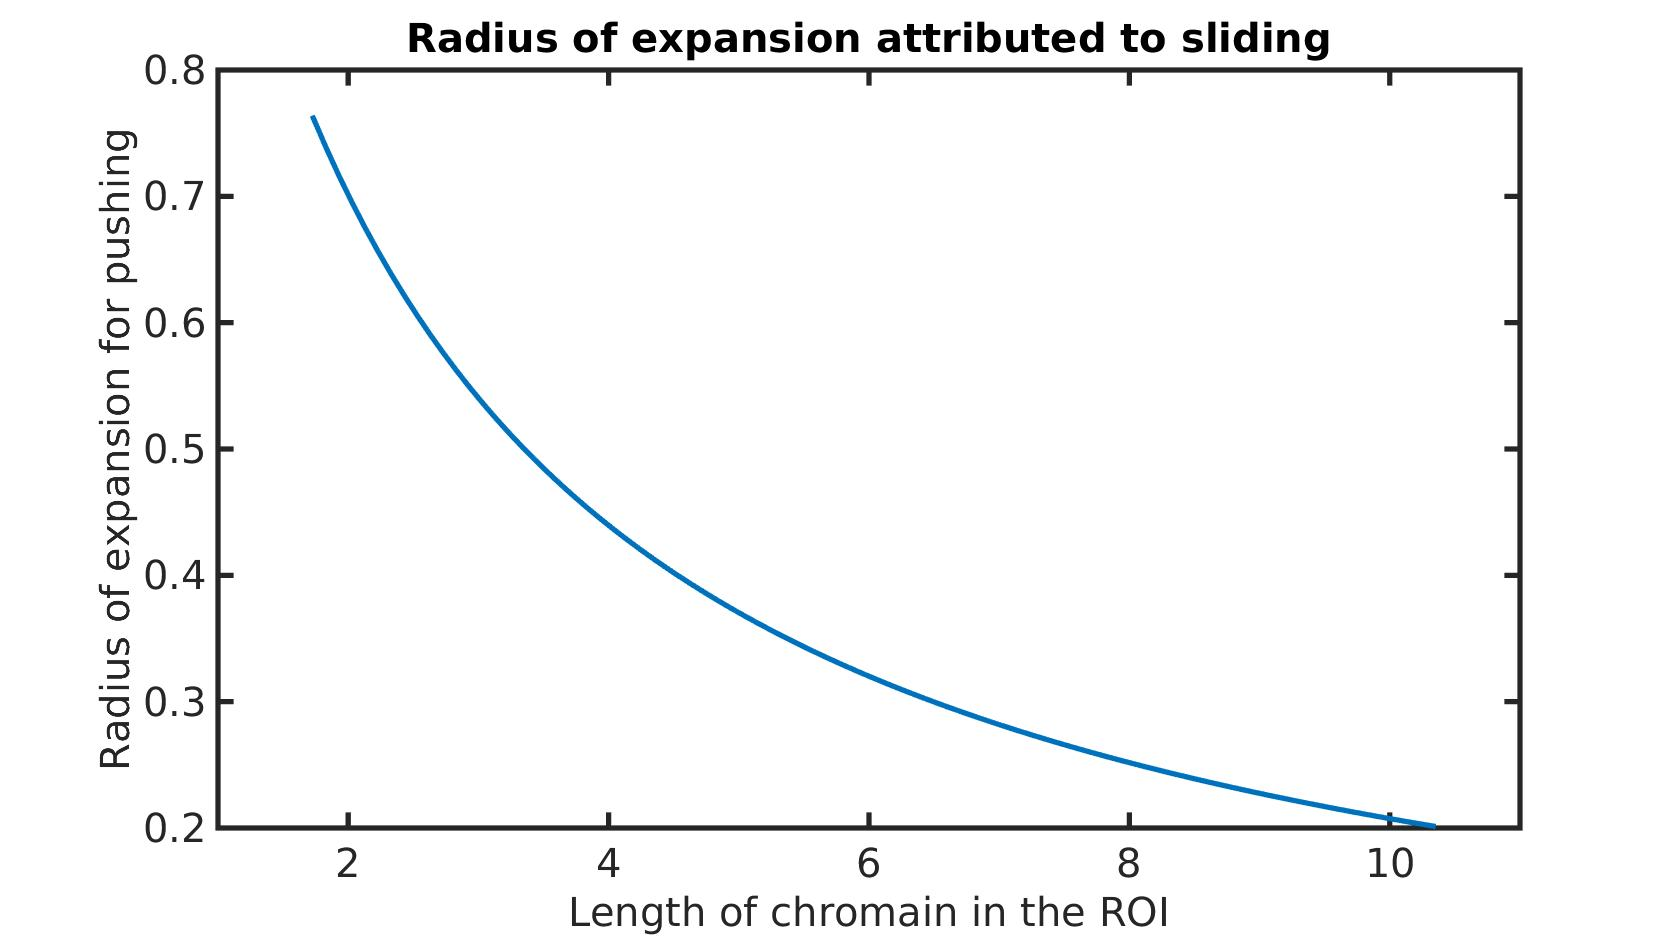
\includegraphics[width=0.5\linewidth, height=0.3\textheight]{Images/SlidingModel/radiusOfSlidingVsLengthOfChromatinInROI}
			\caption{The expansion radius attributed to pushing with no sliding (left) of chromatin as a function of the length of chromatin in the region, and it's complement, the radius of expansion attributed to pushing + sliding (right) as a function of the length of chromatin in the ROI. The ROI expansion is set to $\sqrt{3}$ and values of the chromatin length range from $\sqrt{3}$ to $7\sqrt{3}$}
			\label{fig:radiiVsLengthOfChromainInROI}
		\end{figure}
		
									
		\section{Estimation of the contribution of sliding to the expansion from the data}
		We have no direct access to the length of a single line of chromatin in the ROI. We estimate it indirectly from mass conservation considerations during expansion of the illuminated patch. 
		
		Assuming uniform density of histones before UVC, measurement of the expansion of the patch shows 25-30\% increase in radius (Figure \ref{fig:patchExpansionMeasurement})
		\begin{figure}[H]
			\centering
			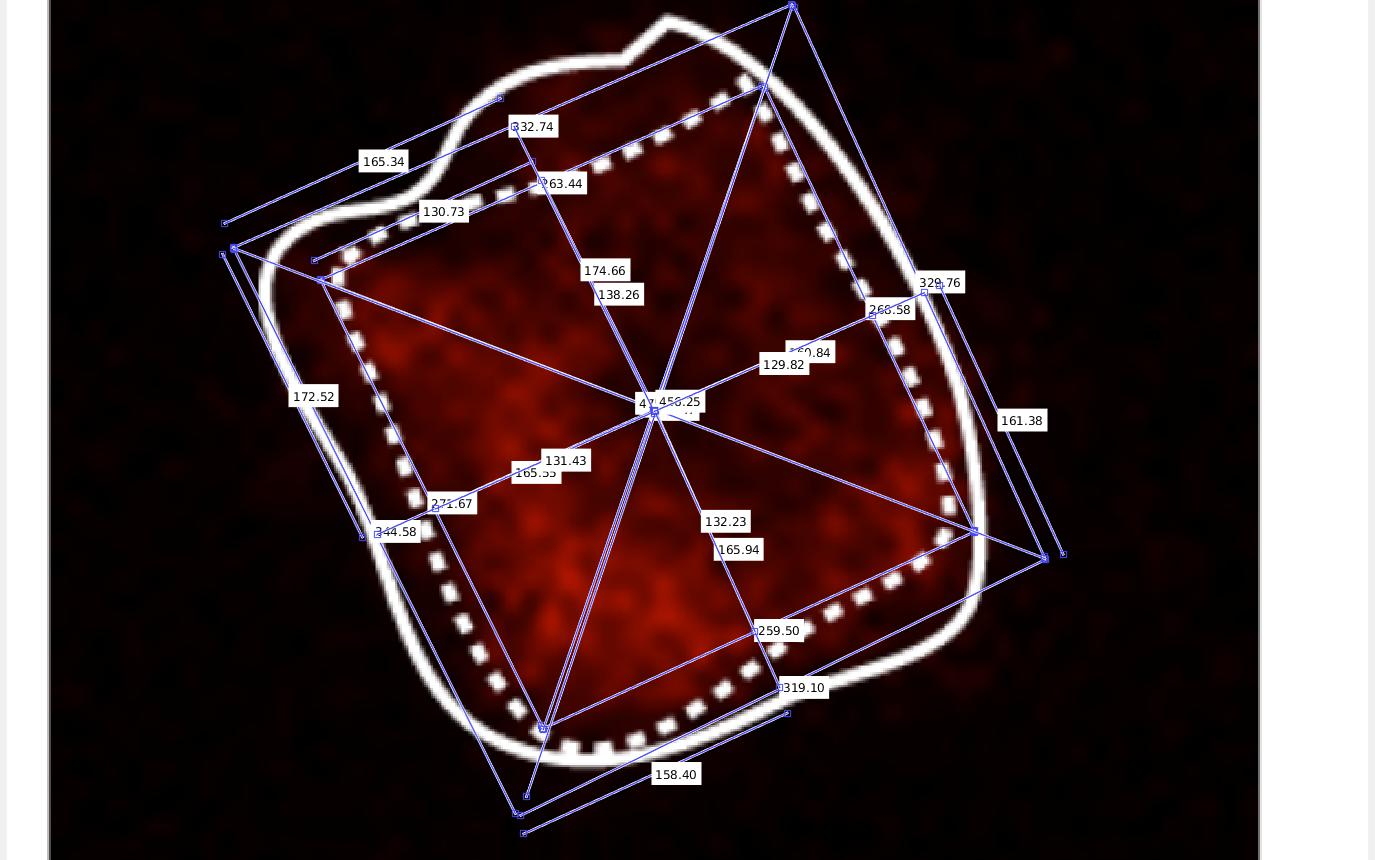
\includegraphics[width=0.5\linewidth, height=0.3\textheight]{Images/PatchExpansion/patchExpansionMeasurement}
			\caption{\tiny{measurement of patch expansion from time 0  just before UVC (dashed) to 15 minutes post UVC (full line) the patch grows by 25-30\% of its initial radius, from 2.52 to the range [3.15,  3.28] }}
			\label{fig:patchExpansionMeasurement}
		\end{figure}
		
		
		\begin{figure}[H]
			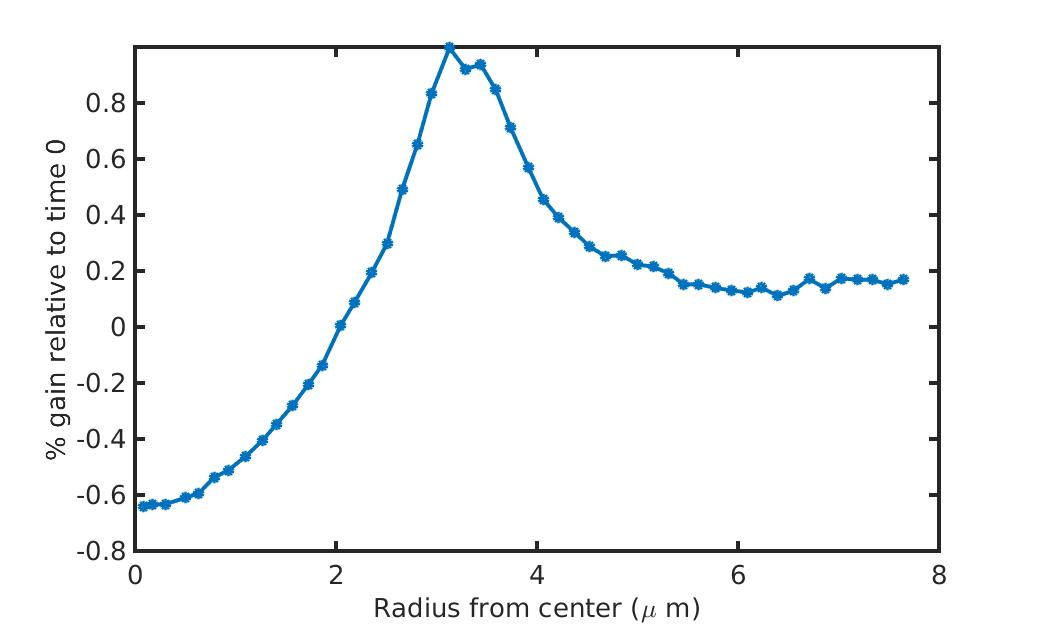
\includegraphics[width=0.5\linewidth, height=0.3\textheight]{Images/PatchExpansion/relativeGainNucleosomesConcentric}
			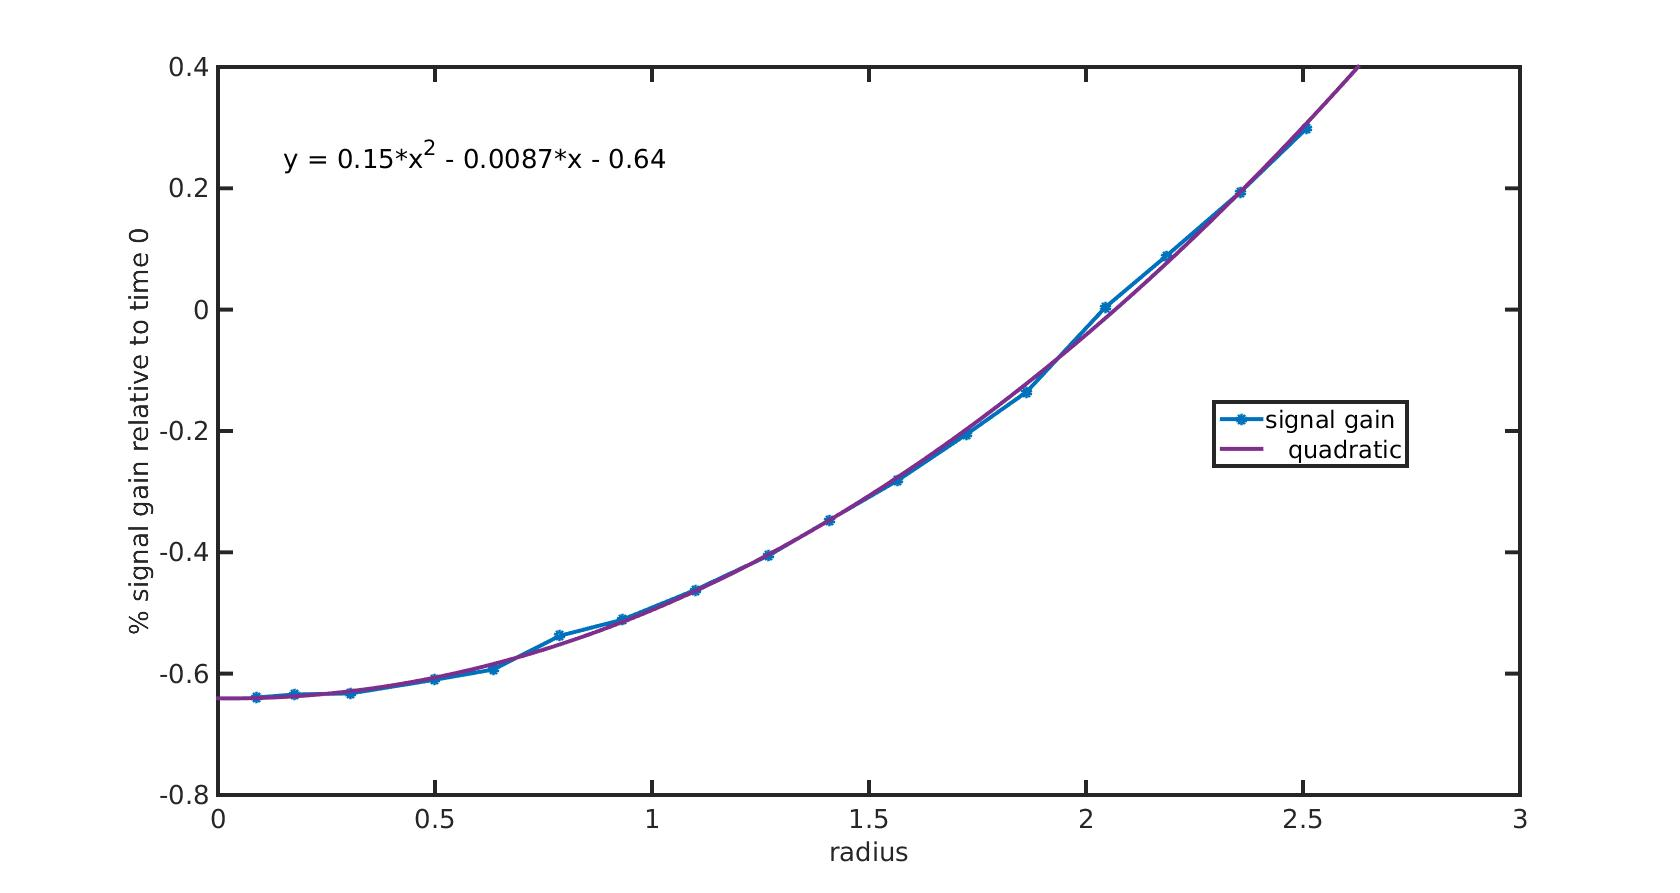
\includegraphics[width=0.5\linewidth, height=0.3\textheight]{Images/PatchExpansion/nucleosomeSignalGainConcentricFit}
			\caption{The relative gain 15 minutes post UVC relative to 0 minutes (left). A fit of the gain function up to the boundary of the patch (right) by a quadratic polynomial}
			\label{fig:relativeGainNucleosomesConcentric}
		\end{figure}
		
		Using 		
		\begin{equation}\label{eq:HistonePreservationConcentric}
		\frac{\int_0^RF(r)(y(r)+1)dr}{\int_0^RF(r)dr} =\gamma
		\end{equation} 
		with $F(r)$ the amount of histones in concentric ring between $r$ and $r+dr$, $y(r)$ the quadratic fit to the gain function, and $\gamma$ is the fraction of histones in a region of radius $R$. We find that the expansion radius attributed to sliding is in the range 0.34 to 0.46 $\mu m$.  
		
		Plugging this estimation in the formula for the $L$ gives us an estimation of the ratio between the ROI radius and the length of DNA in the ROI
		\begin{equation}\label{eq:ratioOfDNALengthToRoiRadius}
		\frac{l}{\beta} = \frac{L\pi(d-h)}{(\beta-L)(d-1)}
		\end{equation}				
		
		\section{Simulation of expansion and repair}
		To examine the organization of the chromatin after repair, we perform simulations of the damage process and expansion. Expansion of 1.7 is obtained for a polymer with 80\% cross-links. 
		
		
\end{document}